\begin{figure*}
\centering
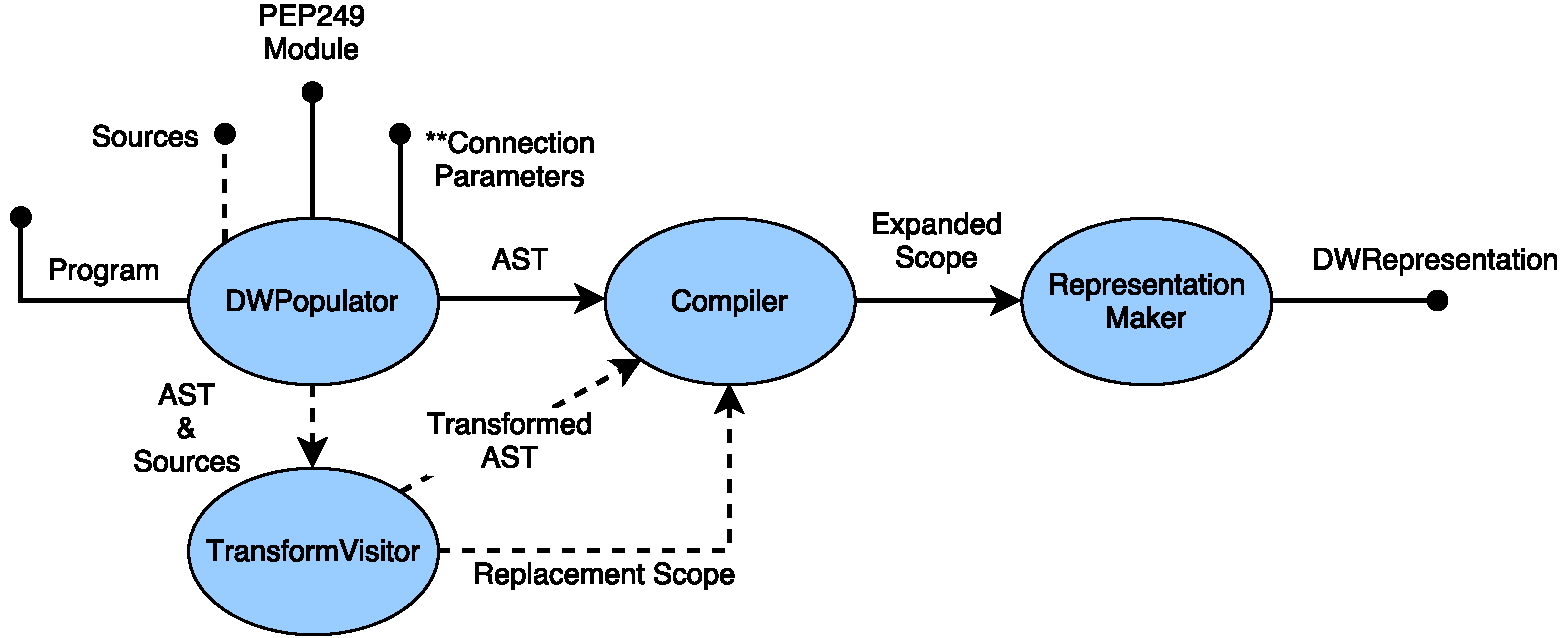
\includegraphics[width=1\textwidth]{figures/reinterpreter.pdf}
\caption{Data flow diagram of the Reinterpreter}
\label{fig:reinterpreter}
\end{figure*}

\section{pygrametl Reinterpreter}

In this section we will describe, in detail, the implementation of the reinterpreter component. Its purpose is to make it easier for users to replace the sources and DW in their pygrametl programs. Users may give test sources and DW as input to the reinterpreter, rather than hardcoding them into the program itself. The reinterpreter also outputs a DWRepresentation object, which describes the structure and contents of the DW in question. On \cref{fig:reinterpreter} is a dataflow diagram which illustrates the flow of data through the reinterpreter. Please note that this depiction is abstracted from the actual implementation to ease explanation. In the following subsections, we will describe each of the four sub-components shown on the figure. Following this we describe what restrictions the component operates according to.

\subsection{ScopeMaker}
The ScopeMaker has the job of connecting to the DW and creating the replacement scope. The input sources are a list of objects used to connect to test sources, which may either be databases or a CSV files. When connecting to a CSV file the object is a file handle, but when connecting to a database it is a PEP249 connection object. From now on, when we refer to a connection object, it means either of these two. The component begins by first instantiating a PEP249 connection object to the DW using the module and connection parameters. The ScopeMaker can then create the replacement scope, as connection objects to both test sources and DW are available . The replacement scope is an ordered dictionary used to replace connections in the pygrametl program. Each source connection object is paired with the key \_\_x\_\_ , where x is the source's index in list incremented by one. The DW connection object is paired with the key \_\_0\_\_. Once completed the replacement scope is sent to the TransformVisitor.

\subsection{TransformVisitor}
The TransformVisitor is a class taking as input the replacement scope and the AST of the pygrametl program being tested. This component is used to walk over the AST, replacing the program's connections with those from the replacement scope. It inherits from ast.NodeVisitor and overwrites the visit\_Call method. This method is called, when a call node implementing a call to a method or function, is encountered. The overwritten method is shown below:

\insertcodefile{codeRelated/scripts/CallNode.py}{The visit\_Call method of TransformVisitor}


The method only reacts to certain pygrametl method calls. After extracting the name of the method being called, we react if the name is contained in either ATOMIC\_SOURCES or WRAPPERS.

ATOMIC\_SOURCES is a list of the non-aggregate sources SQLSource, CSVSource and TypedCVSSource. All other sources from pygrametl.sources are aggregates of these three. Thus there is no reason to react to these. If the method name is contained within ATOMIC\_SOURCES, it means that a non-aggregate source is being instantiated. One of the parameters used for such an instantiation is a connection object. By replacing this with the connection object of a test source, we force the non-aggregated source to point at the test data. This means that the object can now be used to access test data, rather than the data it was hardcoded to do. The replacement process itself consists of replacing the hardcoded connection parameter with a dummy key from the replacement scope. For the first source encountered the key will be \_\_1\_\_, the second \_\_2\_\_ and so on. These will later be used as identifiers, when executing the AST.

WRAPPERS contains only ConnectionWrapper from pygrametl.init. This is the class used to access DWs with pygrametl. Once the instantiation of a ConnectionWrapper is encountered, we simply replace its connection parameter with the key \_\_0\_\_, pointing to the test DW in the replacement scope. We also set a flag that makes sure that we raise an exception if another ConnectionWrapper is encountered. We do this to restrict \FW{} to only work with pygrametl programs that function on a single DW.

Once the entire tree has been walked, a transformed AST has been produced. This tree along with the replacement scope is now sent to compilation.


\subsection{Compiler}
In this component we compile and execute the transformed AST using the replacement scope as its local scope. This is done with calls to the build in python functions compile and exec. In python, a scope is given by a dictionary, where keys are variable names paired with object references. As we replaced the connecting objects in the transformed AST with keys from our own scope, we now force the program to use the test objects from the replacement scope. This way, we overwrite the hardcoded sources and DW from the program. Once the AST has been executed, the test DW will be populated, and the replacement scope expanded with the variables found in the executed pygrametl program. The expanded scope is sent to the RepresentationMaker. After execution we also make sure to reestablish connection to the test DW, in case it was closed during execution.

\subsection{RepresentationMaker}
Using the expanded scope, the RepresentationMaker accesses all Dimension and FactTable objects instantiated through the execution of the pygrametl program. From this it creates a DWRepresentation object that allows for easy access to all the tables of the DW along with their metadata. It begins by instantiating the RepresentationMaker, then calling its run method to create the DWRepresentation object. This method can be seen below:

\insertcodefile{codeRelated/scripts/representation_maker.py}{The run method of the representation\_maker class}

In this method we access the \_alltables list from our scope. Every pygrametl Dimension and FactTable object instantiated during execution of the pygrametl program is logged in this list. Once acquired we iterate over the list and create a representation object for each table. check\_table\_type is a method that returns true, if the table in question has a type contained in a given list. DIM\_CLASSES contains the class names of all non-aggregate Dimension classes from pygrametl.tables. Similarly FT\_CLASSES contains all non-aggregate fact table classes with the exception of SubprocessFactTable. Once the type of a table has been identified relevant metadata such as table name and keys are extracted from the object and used to instantiate a DimenstionRepresentation or FactTableRepresentation respectively and stored in a list. After iteration we identify all SnowflakedDimension objects in our scope and store them in a list. These provide some assistance in discovering the structure of the DW. Afterwards the DWRepresentation object is instantiated with the two lists of tables, the list of SnowflakedDimensions and the PEP249 connection object connecting to the DW.

Once instantiated, the DWRepresentation is returned to be used by the predicates and the reinterpretation process is completed.

\subsection{Restrictions}
As the dynamic alteration of code can become rather complex if each edge case is considered, we decide to restrict the format of pygrametl programs that can be run through the reinterpreter. As mentioned previously, the program may only function on a single DW. We make this restriction as it makes implementation easier, while the use of more than one DW is uncommon. In the RepresentationMaker we also restrict ourselves from extracting meta data from instantiations of the SubprocessFactTable class. This class is used to write data to some sub processes such as a bulkloader. We ignore it, as it does not contain the needed metadata such as a table name. As we replace connections by walking over the AST, programs may not instantiate several source or table objects through iteration. This is because a AST walker only moves over the code within a loop a single time. Finally, the instantiation of pygrametl sources and tables may only occur in the script given to the reinterpreter. Imports are still usable, but because the AST walker only traverses the given script, replacements will not be performed inside imported modules.   

